\paragraph{Dispatcher Service}
The dispatcher is a service responsible for handling the communication with the client. It consist of a asynchronous IO and the dispatcher itself. Communication is done by an XML interface where requests from the client is verified by the dispatcher and passed to either the Admin module or a Game Thread depending on the message. 

\paragraph{Logic Layer}
This layer represent the business logic of the server application. The Admin module handles user creation, user login and game creation and is general for all game implementations. Game Thread is where specific game logic is implemented and its implementation will vary depending on the type of game. Event Timer is a general module handling events specified to happen at certain times. The game threads are responsible for creating events for themselves. The event timer will then notify a game thread at the specified time.

\paragraph{Data Layer}
Is the database representation in the model using the data mapper pattern\fxwarning{WE book ref}. The gateway is responsible for querying and updating the database and mapping the tables to objects used in the game logic and administration.

\begin{figure}[H]
  \centering
  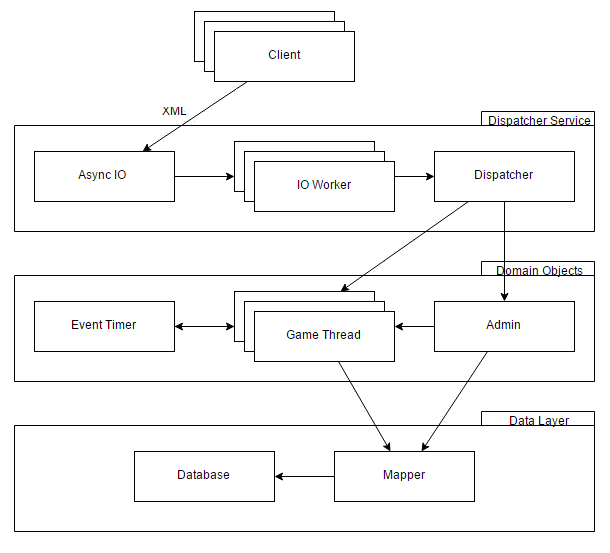
\includegraphics[width=\textwidth]{billeder/serverarch.png}  
  \caption{Architecture of server displaying the branching of an incoming connection}
  \label{fig:serverarch}
\end{figure}